\documentclass{article}

\usepackage{kern}

\begin{document}
    \subsection{Rauschanalyse}\label{subsec:3:Rauschanalyse}
    Um das Maximum der Rauschkurve zum Schwingkreis zu erhalten und die Resonanzfrequenz abzuschätzen, verwenden wir eine Kurvenanpassung mithilfe der gegebenen Normalverteilungsfunktion $f_G$ zu den Parametern $a,\, b,\, c,\, d\in\R$ der Form
    \[
        f_G(x) := a\cdot\exp(-\frac{1}{2}\cdot\nbra{\frac{x + b}{c}}^2) + d.
    \]
    Dabei korreliert $c$ zur Standardabweichung $\sigma(f_G)$ der Normalverteilung und $b$ zur Lage des Maximums $x_0$. Den Vorfaktor $1/(\sigma\cdot 2\pi)$ der allgemeinen Definition verpacken wir in $a$. Als Visualisierung der Anpassungsgenauigkeit ziehe Abbildung \ref{fig:3:GaussFit1} herbei. \\
    Zur Beschreibung der Breite des Peaks ziehen wir die Methode der Halbwertsbreite (\emph{full width at half maximum}, FWHM) heran. Diese ist definiert als die Differenz der beiden Punkte, an denen die Funktion den halben Maximalwert annimmt. Für die Gaußfunktion $f_G$ mit Maximalwert $f_G(x_0) = \max(f_G)$ und Standardabweichung $\sigma(f_G)$ gilt
    \[
        \text{FWMH}(\sigma(f_G)) := 2\cdot\sqrt{2\cdot\ln(2)}\cdot\sigma(f_G).
    \]
    Als Unsicherheit $(u\circ\text{FWMH})(f_G)$ erhalten wir durch Richtungsableitung $d\text{FWMH}(\sigma(f_G))((u\circ\sigma)(f_G)) = 2\cdot\sqrt{2\cdot\ln(2)}$ mit $f_G$ als einzige Variable das skalierte Ergebnis \cite[wiki]{enwiki:FWHM}
    \[
        (u\circ\text{FWHM})(f_G) = \ubra{2\cdot\sqrt{2\cdot\ln(2)}}{=:c}\cdot (u\circ\sigma)(f_G).
    \] 
    Die Auswertung der Daten anhand dieser Zusammenhänge liefert uns die folgende Übersichtstabelle \ref{tab:3:PeakInfo}.
    \begin{table}[H]
       \centering
       \begin{tabular}{c|ll|ll}
            \textbf{Durchgang} & $\max(f_G)$ & $(u\circ\max)(f_G)$ & $\text{FWHM}(f_G)/c$ & $(u\circ\text{FWHM})(f_G)/c$ \\
            \hline
            1 & $2008.75$ & $8.64$ & $119.46$ & $9.28$ \\
            2 & $2006..68$ & $7.75$ & $112.324$ & $8.28$ \\
            \hline
            avg. & $2007.715$ & $11.61$ & $115.892$ & $12.44$
        \end{tabular} 
        \caption{Resonanzpeakanalyse anhand eines Gauß Fits.}
        \label{tab:3:PeakInfo}
    \end{table}
    Die einzelnen Unsicherheiten ergeben sich durch die asymptotische Standardabweichung der Kurvenanpassung. Das aufkommende Rauschen besitzt nach der verwendeten Prospa Software einen \emph{root mean square} (rms) von $8.7\si{\micro\volt}$ ohne Bekannte Unsicherheit, stimmt jedoch mit der Standardabweichung $\sigma = 8.6841$ des Rauschdatensatzes überein. \\
    \begin{figure}[H]
        \centering
        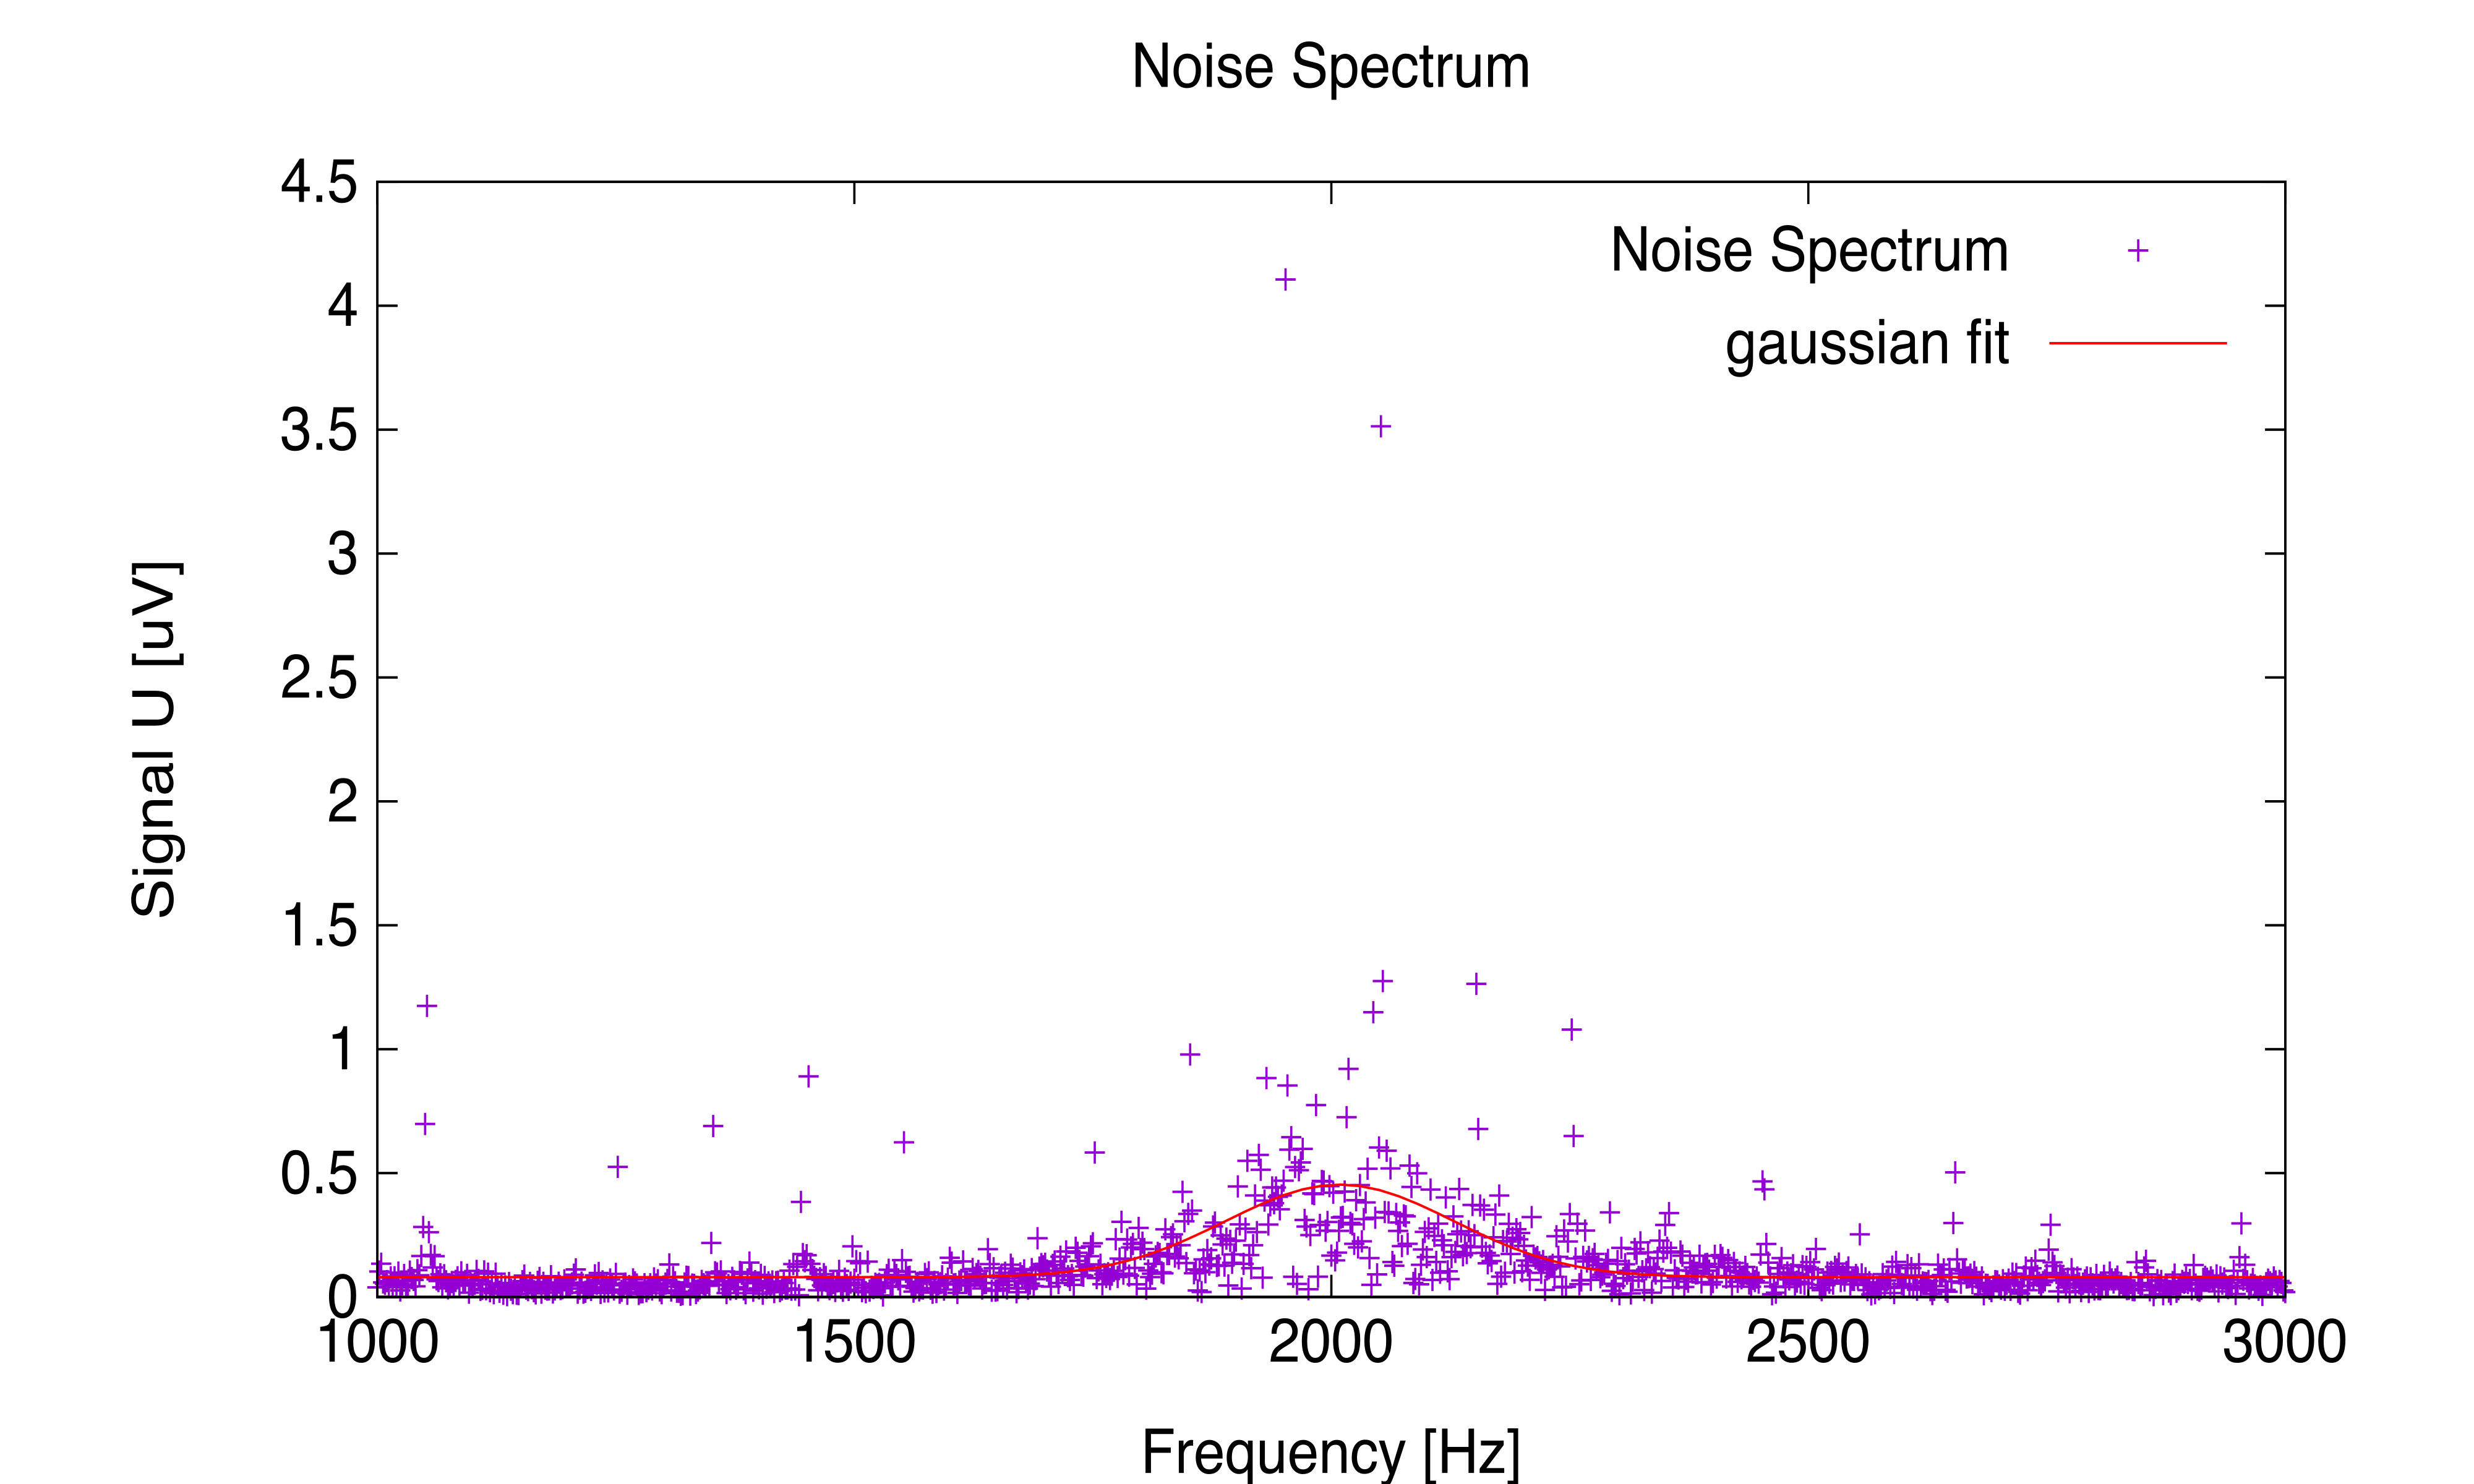
\includegraphics[width=10cm]{../Bilddateien/Messung1_Noise_Spectrum_Gaussian.png}
        \caption{Gaußanpassung an die Rauschkurve des Schwingkreises für Durchgang 1.}
        \label{fig:3:GaussFit1}
    \end{figure}
    Betrachten wir die in Kapitel \ref{sec:2:LarmorBestimmungWasser} bestimmte Larmorfrequenz, so liegen LC-Schwingkreis Resonanzfrequenz und selbige bereits dicht beieinander. Dies deutet auf bereits gut gewählte Startwerte in der Konfiguration \ref{fig:3:MonitorNoiseConfig} hin. 
    \begin{figure}[H]
        \centering
        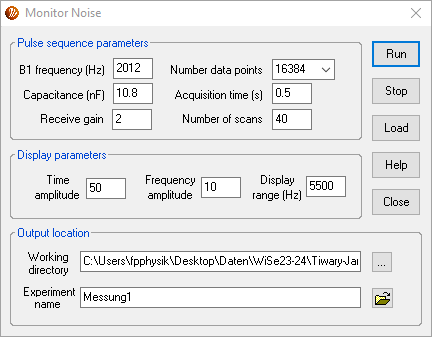
\includegraphics[width=8cm]{../Bilddateien/Sec3_Monitor_Noise_Configuration.png}
        \caption{Konfiguration der Messung der Rauschkurve des Schwingkreises.}
        \label{fig:3:MonitorNoiseConfig}
    \end{figure}
    Betrachtet man das Spektrum einmal in einem größeren Frequenzintervall, so sind wie in Abb. \ref{fig:3:NoiseSpectrum} ersichtlich mehrere Nebenpeaks in empirischen Abständen von $50\si{\herth}$ zu erkennen. Diese sind auf die Netzfrequenz von $50\si{\hertz}$ zurückzuführen. Dieses als \emph{Oberschwingungen} bekannte Phänomen ist in erster Linie auf die im Versuchsaufbau verwendeten Kabel und Kondensatoren, sowie weitere elektrische Bauteile zurückzuführen \cite[TÜV]{TUEV:Oberschwingungen}.
    \begin{figure}[H]
        \centering
        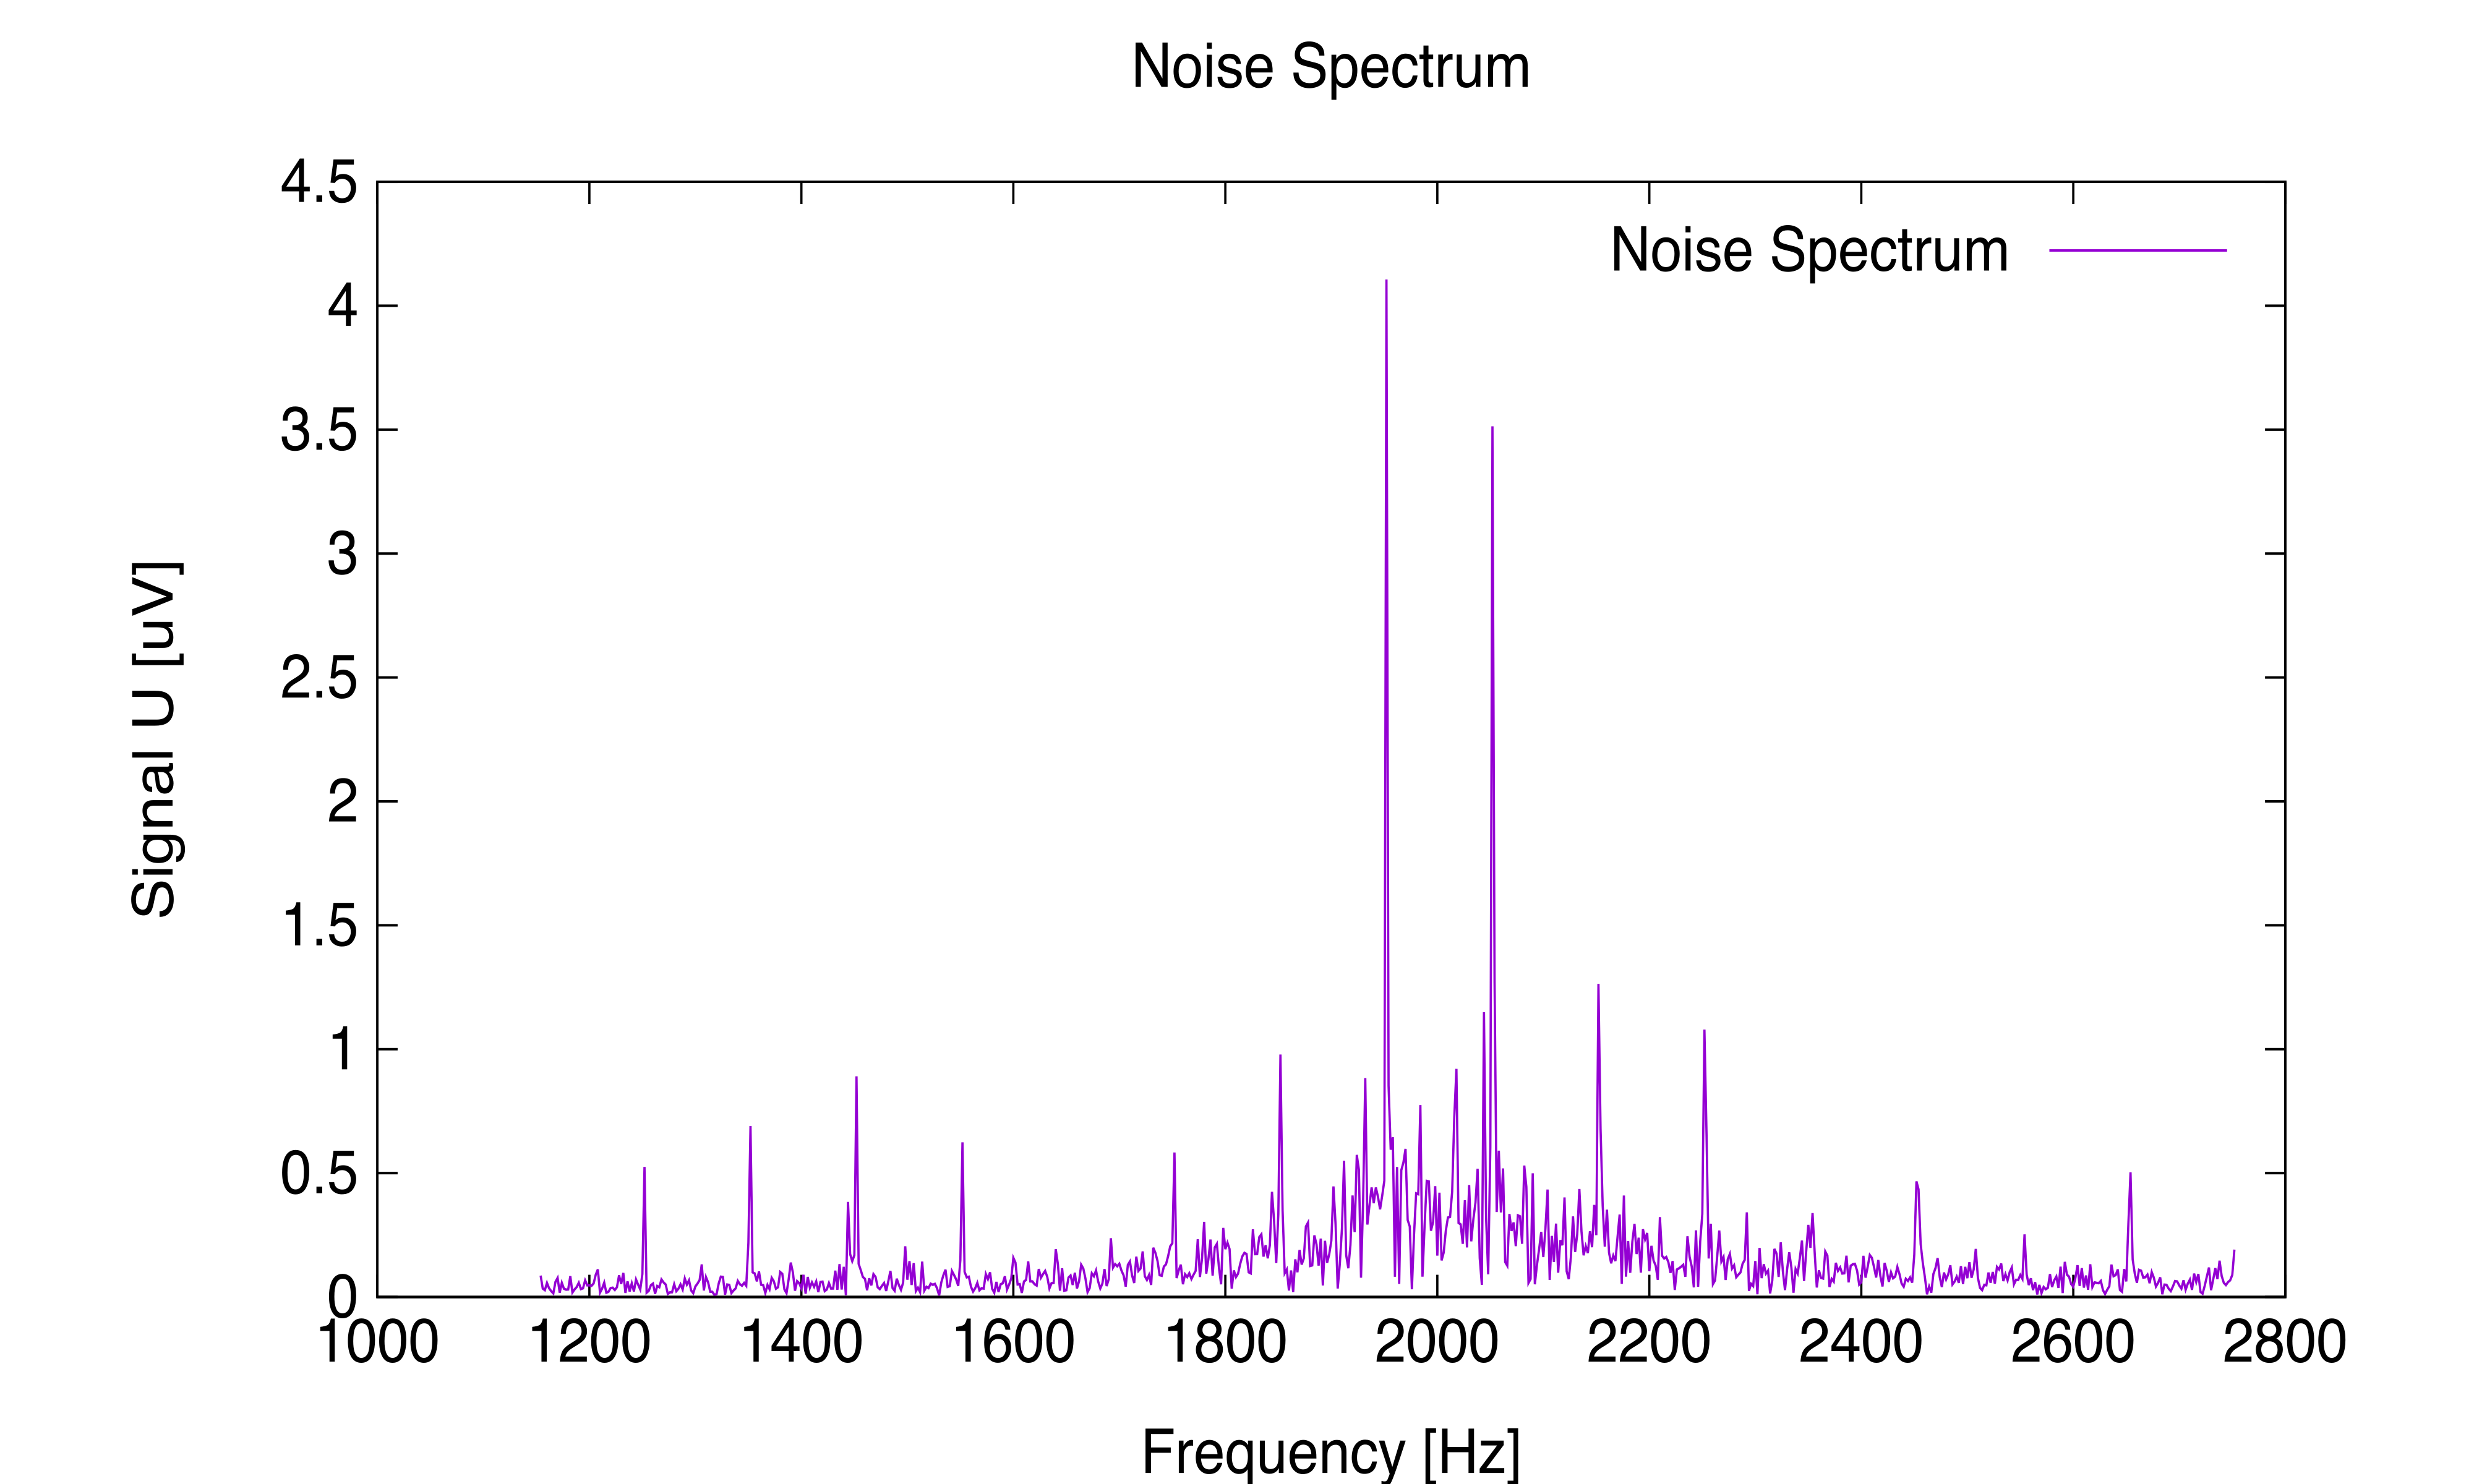
\includegraphics[width=10cm]{../Bilddateien/Messung1_Noise_Spectrum.png}
    \end{figure}

    \bibliography{../Literatur.bib}
\end{document}